\documentclass[11pt]{article}
\usepackage[margin=0.70in]{geometry}
\usepackage{booktabs}
\usepackage[colorlinks=true,linkcolor=blue,citecolor=blue,urlcolor=blue]{hyperref}
\usepackage[shortlabels]{enumitem}
\usepackage{longtable}
\usepackage{graphicx}
\usepackage{subcaption}
\linespread{0.95} % Reduce overall line spacing
\setlength{\parskip}{0.5em} % Reduce vertical space between paragraphs
\setlength{\parindent}{0pt}

\begin{document}

\begin{center}
    {\Large\textbf{Andrew James Steinmetz, Ph.D.}}\\[0.5em]
    {\large\textbf{Research Statement}}
\end{center}

My research program (with collaborators at University of Arizona, ELI-Beamlines ERIC, Wigner RCP, and Texas U.) rigorously investigates spin and magnetic moments in relativistic mechanics, addressing both quantum and classical regimes. Central to my work is the special role of the gyromagnetic ratio (g-factor), anomalous magnetic moment (AMM), and its connection to the algebraic structure of spin. This is then used to explore classical, quantum, and macroscopic astrophysical processes; see \href{http://hdl.handle.net/10150/670301}{Steinmetz, (2023)}. I am either the author, or co-author, of all included references.

{\large\textbf{Quantum Investigations: Relativistic Spin Dynamics and Magnetism}}\\
We have studied generalizations of arbitrary magnetic moments for fermions (\href{https://doi.org/10.1088/1361-6587/aac06a}{Formanek et al., 2018}). In particular, we investigated the second-order fermion Klein-Gordon-Pauli (KGP) equation (\href{https://doi.org/10.1140/epja/i2019-12715-5}{Steinmetz et al., 2019}) in the following cases:
\begin{itemize}[leftmargin=1.5em,nosep]
    \item \emph{Homogeneous Magnetic Fields:} We examine solutions of generalized second-order fermions in uniform fields, emphasizing the impact of the AMM on the energy spectrum.
    \item \emph{Hydrogen-like Atoms:} We extended the Coulomb problem to include AMM effects from KGP, thereby elucidating corrections to atomic spectra for high-\(Z\) systems; see Figure~\ref{fig:figure1}.
    \item \emph{Mass-Magnetic Moment Coupling:} We explore alternative approaches that couple mass with magnetic moment, providing new insights into relativistic quantum behavior.
\end{itemize}
Our work emphasizes the often-overlooked distinction between the KGP and the Dirac equations, as they present different physical solutions when AMM is present.

{\large\textbf{Classical Models: A Covariant Stern-Gerlach Framework}}\\
On the classical side, my collaborators and I proposed a relativistic covariant model of the Stern-Gerlach force by introducing a magnetic four-potential. This framework \href{https://doi.org/10.1140/epjc/s10052-017-5493-2}{Rafelski et al., (2018)} covers:
\begin{itemize}[leftmargin=1.5em,nosep]
    \item \emph{Extended BTMT Equations:} We modify the standard covariant Thomas-Bargmann-Michel-Telegdi (TMBT) torque equations and introduce a novel secondary AMM that follows a different covariant structure than the traditional AMM.
    \item \emph{Ampèrian and Gilbertian Equivalence:} In this covariant framework, we unite the Ampèrian and Gilbertian descriptions of magnetic moments and show that the distinction between them can be understood in terms of external four-currents.
\end{itemize}
This model resolves longstanding ambiguities in the classical treatment of magnetic dipoles and provides a robust platform for further experimental and theoretical exploration. It has led to improved understanding of covariant motion in plane-waves for both charged and neutral particles (\href{https://doi.org/10.1088/1361-6587/ab242e}{Formanek et al., 2019}; \href{https://doi.org/10.1103/PhysRevD.102.056015}{Formanek et al., 2020}; \href{https://doi.org/10.1103/PhysRevA.103.052218}{Formanek et al., 2021}).

{\large\textbf{Neutrino Physics: Electromagnetic Flavor Mixing}}\\
Extending these principles to neutrino physics, we have focused on (transition) magnetic dipoles in Majorana neutrinos. Key points developed in \href{https://doi.org/10.1142/S0217751X23501634}{Rafelski el al., (2023)} include:
\begin{itemize}[leftmargin=1.5em,nosep]
    \item \emph{EM-Induced Flavor Mixing:} We explicitly demonstrate electromagnetic flavor mixing in a two-flavor neutrino model, showing that flavor mixing can be dynamically produced in strong electromagnetic field regimes.
    \item \emph{Dynamical Mass Basis:} Building on earlier work, we developed an EM rotation matrix that defines a dynamical mass basis, allowing a direct comparison of EM-induced neutrino mass splitting with the observed neutrino mass hierarchy.
\end{itemize}
This work offers a novel perspective on the interplay between electromagnetic fields and neutrino properties, with potential implications for understanding neutrino behavior in astrophysical environments.

{\large\textbf{Cosmological Applications: Primordial Magnetization}}\\
Applying our theoretical developments to cosmology (\href{https://doi.org/10.3390/universe9070309}{Rafelski et al., 2023}; \href{https://doi.org/10.48550/arXiv.2409.19031}{Rafelski et al., 2025}), we proposed a model for magnetic thermal matter-antimatter plasmas. In this model of spin-polarized plasmas, we examined:
\begin{itemize}[leftmargin=1.5em,nosep]
    \item \emph{Electron-Positron Epoch:} We investigated the paramagnetic characteristics of electron-positron plasma subjected to an external primordial field, suggesting that the origin of primordial magnetic fields (PMF) may be related to the spin polarization of the hot dense plasma despite conventional wisdom that high temperatures disrupt magnetization (\href{https://doi.org/10.1103/PhysRevD.108.123522}{Steinmetz et al., 2024}).
    \item \emph{QGP Epoch:} We studied spin magnetization during the quark-gluon-plasma (QGP) epoch and estimated maximum bounds for spin magnetization; see Figure~\ref{fig:figure2}. We also suggested that electromagnetic-color dipole interactions could drive polarization prior to hadronization (\href{https://doi.org/10.48550/arXiv.2502.05052}{Steinmetz \& Rafelski, 2025}).
\end{itemize}
This research indicates that even a small polarization asymmetry in the plasma can generate magnetic fields with strengths consistent with those observed in deep intergalactic space. Further work has also improved the theory of fermion statistics in different temperature regimes (\href{https://doi.org/10.1007/s10773-024-05695-8}{Birrell et al., 2024}).

{\large\textbf{Future Research Goals and Projects}}\\
Building on our established work, I am actively pursuing several projects in various stages of development:
\begin{itemize}[leftmargin=1.5em,nosep]
    \item \emph{Strong Fields in Classical and Quantum Physics Review:} (in preparation, 2025) A comprehensive review synthesizing recent advances and our contributions across classical and quantum domains. The first draft is complete and under internal revision.
    \item \emph{Magnetized Primordial Quark-Gluon Plasma:} (first author, in preparation, 2025) A follow-up to \href{https://doi.org/10.48550/arXiv.2502.05052}{Steinmetz \& Rafelski, (2025)} investigating the role of magnetic fields during the QGP epoch with further theoretical and numerical developments of early-universe magnetization processes around hadronization.
    \item \emph{Electromagnetic Field Forcing of Dynamic CP-Violation in the Lepton Sector:} (first author, in preparation, 2025) A study addressing how strong electromagnetic fields can induce dynamic CP-violation in the lepton sector, with potential implications for physics beyond the Standard Model.
    \item \emph{Anomalous Magnetic Moment in the QCD Vacuum:} (in preparation, 2025) An analysis focused on the behavior of anomalous magnetic moments within the QCD vacuum, emphasizing underlying non-perturbative QCD effects.
\end{itemize}
Future work will focus on hadronic physics in high-energy experiments and early universe cosmology, furthering our understanding of spin dynamics, strong-field effects, and non-perturbative QCD phenomena.

{\large\textbf{Select Figures}}\\
I produced the following figures in the course of research which are examples of key theoretical results.
\begin{figure}[h!]
    \centering
        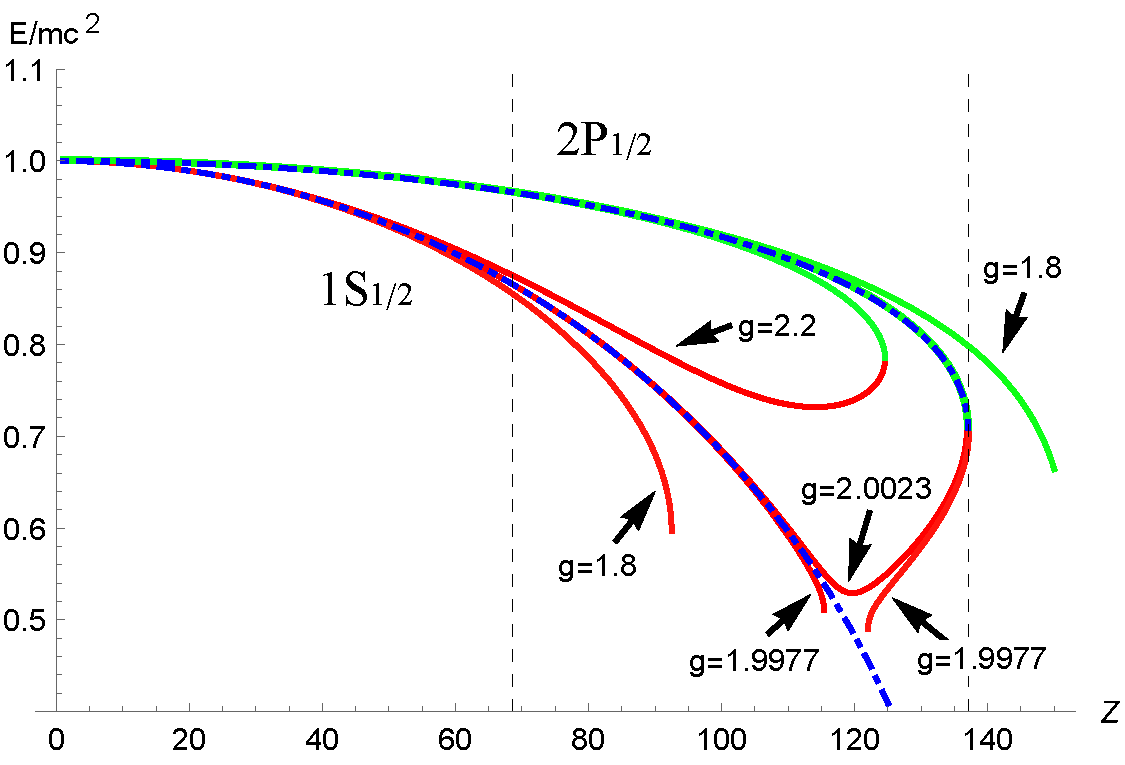
\includegraphics[width=0.44\linewidth]{lanplot08.pdf}
        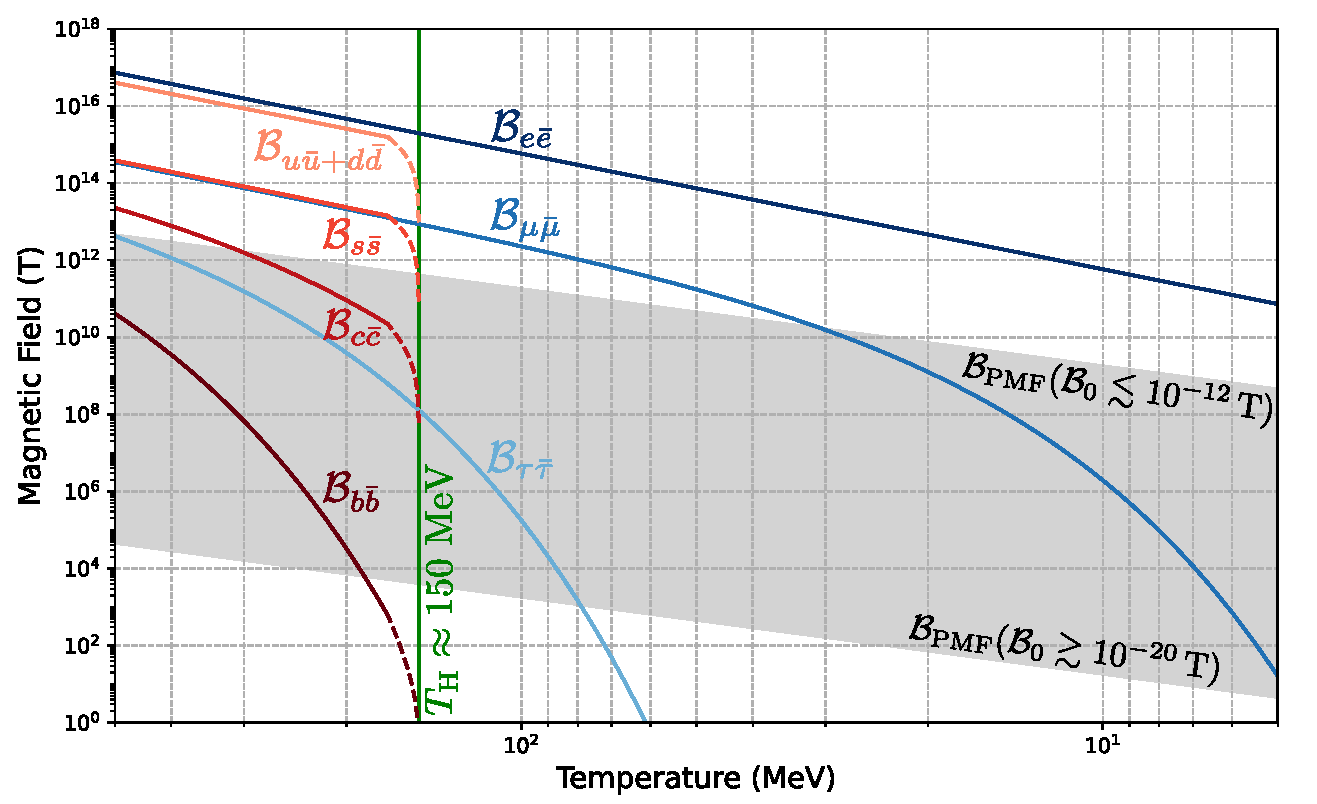
\includegraphics[width=0.54\linewidth]{Figure_1_v3.pdf}
    \caption{(Left) The KGP 1S\(_{1/2}\) (red) and 2P\(_{1/2}\) (green) energy states for a hydrogen-like atom for differing values of the g-factor are compared to the Dirac result (dashed blue); reprinted from \href{https://doi.org/10.1140/epja/i2019-12715-5}{Steinmetz et al., (2019)}.}
    \label{fig:figure1}
    \caption{(Right) The maximum spin magnetization for leptons and quarks is shown before and after hadronization at approximately 150~MeV. The grey band indicates the estimated PMF strength based on contemporary intergalactic magnetic field measurements and conservation of magnetic flux; reprinted from \href{https://doi.org/10.48550/arXiv.2502.05052}{Steinmetz \& Rafelski, (2025)}.}
    \label{fig:figure2}
\end{figure}

\newpage

\begin{center}
    {\Large\textbf{Andrew James Steinmetz, Ph.D.}}\\[0.5em]
    {\large\textbf{Teaching Statement}}
\end{center}

My goal as an educator is to foster an intuitive understanding of the universe, both for myself and for my students. The mutual exchange of enthusiasm between myself and students creates a uniquely rewarding environment. I have been fortunate to teach students at the University of Arizona (UA), the Arizona College of Technology at Hebei University of Technology (ACT/HEBUT), and Pima Community College (PCC).

Students often grapple with personal anxiety, cultural differences, and unfamiliarity before fully engaging with the material. To overcome these barriers, I consistently present unshakable enthusiasm and a genuine interest in the subject matter. To keep student interest high, I tie theoretical topics to concrete examples or research data. I especially appreciate hearing from students when their perception of science has improved, a sentiment that resonates across all levels, from introductory courses to advanced courses.

{\large\textbf{Active Learning and Instructional Methods}}\\
My teaching style has evolved toward active learning, blending traditional lectures with in-class group activities. I organize students into small groups of three to five, encouraging them to work together repeatedly on challenges throughout the semester. I provide my students with detailed supplementary material such as relevant videos, images, computer programs, or experimental data relevant to the topics being covered. This approach emulates the participatory nature of laboratory courses using pen-and-paper exercises, while also reinforcing teamwork skills essential for future careers. 

A modern challenge for instructors is the rise of AI tools like ChatGPT, which can solve even complex upper-level physics problems. To address this, I emphasize in-class evaluations and collaborative exercises to design assessments that remain meaningful and resilient to these technological shifts. I track student performance on exams by doing statistics on which topics they score well on versus those they have difficulty with and adjust my teaching throughout the year to compensate.

{\large\textbf{Diverse Teaching Experiences and Adaptability}}\\
My teaching journey spans diverse class sizes and student demographics, from smaller personalized classes at PCC to larger lecture and lab-based courses at ACT/HEBUT, where English is a second language for all students. During the COVID-19 pandemic, I was tasked with scripting and producing videos to explain and demonstrate undergraduate lab experiments. 

In addition to classroom teaching, I regularly advise students on graduate school applications and provide letters of recommendation. I even initiated an undergraduate physics journal club at ACT to discuss advanced topics and research with highly motivated students.

{\large\textbf{Curriculum, Course Development, and Public Outreach}}\\
I have also had the opportunity to develop new courses at ACT/HEBUT. The UA physics curriculum includes two semesters of Experimental Methods in Physics (PHYS 381/382), an upper-level course that was not offered at HEBUT when I arrived in Spring 2024 to Tianjin, China. To implement these courses, I collaborated with laboratory managers, equipment vendors, and contractors (communicating mostly in Chinese via a translator) to refurbish a laboratory room and acquire equipment under tight deadlines.

Designing these courses involved balancing theoretical rigor with practical skills, ensuring that experiments aligned with the UA curriculum while addressing the unique needs of ACT/HEBUT students. I also co-developed a Senior Design/Capstone course that emphasized career skills and group work in an engineering context. Outside the classroom, I enjoy sharing science with the public by uploading astrophotography to \href{https://www.astrobin.com/users/djinn/}{AstroBin}, discussing research on \href{https://bsky.app/profile/ajsteinmetz.com}{BlueSky}, and posting blog entries on my \href{https://ajsteinmetz.github.io/}{personal website}.

\end{document}
